\documentclass{article}

\usepackage{graphicx}
%\usepackage{geometry}
\usepackage{placeins} % use float barriers
\usepackage{float}
\usepackage{subcaption}
\usepackage{longtable}
\usepackage[a4paper,margin=1in]{geometry}
\usepackage{grffile}
\usepackage{multirow}

\title{RL benchmark for the reaching task}
\date{}

\begin{document}

\maketitle


\section{Introduction and methods}

A2C with Pendulum-V0 and 100 000 timesteps + 10 seeds
check 1 to 8 env
check normalise or not

\section{Results}

\subsection{Learning curves}

\begin{figure}[H]
    \centering
    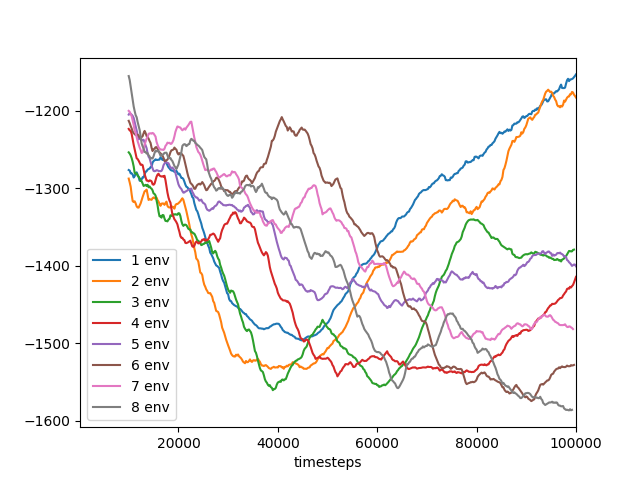
\includegraphics[width=0.7\textwidth]{../learning_curves_by_env.png}
\caption{Learning curves by nb of env.}
\end{figure}

\begin{figure}[H]
    \centering
    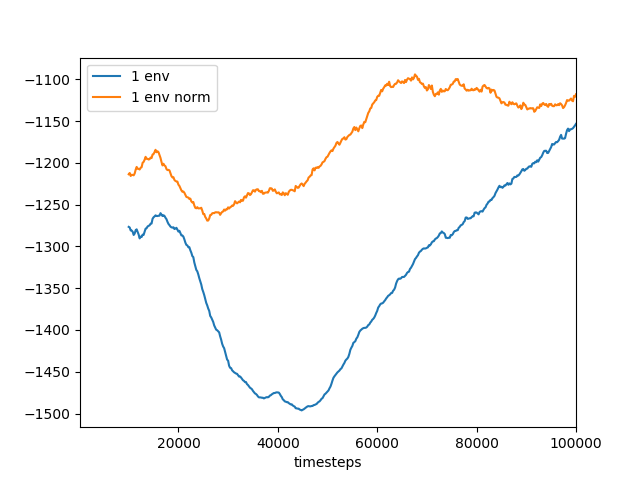
\includegraphics[width=0.7\textwidth]{../learning_curves_norm1.png}
\caption{Learning curves when normalising or not with 1 env.}
\end{figure}

\begin{figure}[H]
    \centering
    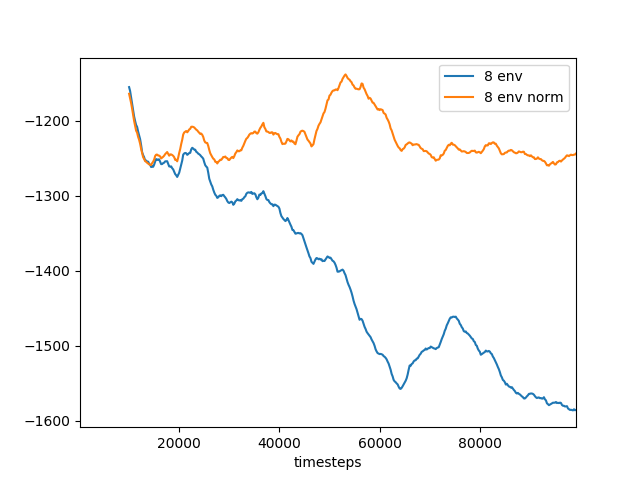
\includegraphics[width=0.7\textwidth]{../learning_curves_norm8.png}
\caption{Learning curves when normalising or not with 8 env.}
\end{figure}



\subsection{Evaluation}


\begin{figure}[H]
    \centering
    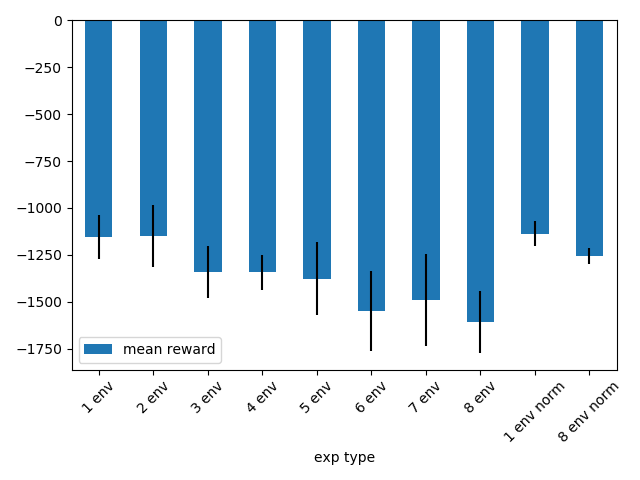
\includegraphics[width=0.7\textwidth]{../reward_by_exp_type.png}
\caption{Reward vs env type.}
\end{figure}

\begin{figure}[H]
    \centering
    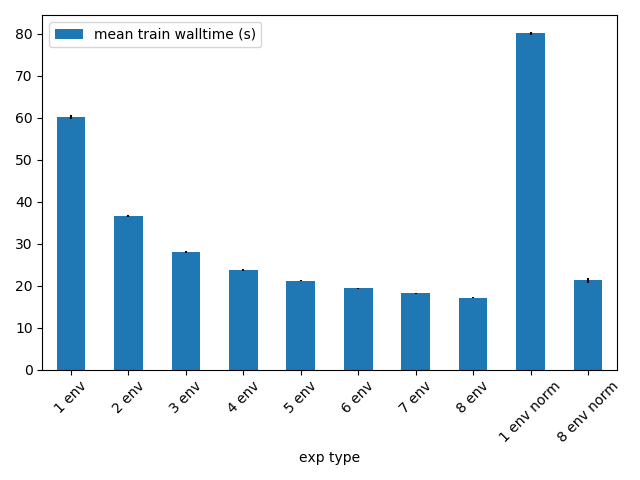
\includegraphics[width=0.7\textwidth]{../train_time_by_exp_type.png}
\caption{Train time vs env type.}
\end{figure}

\begin{figure}[H]
    \centering
    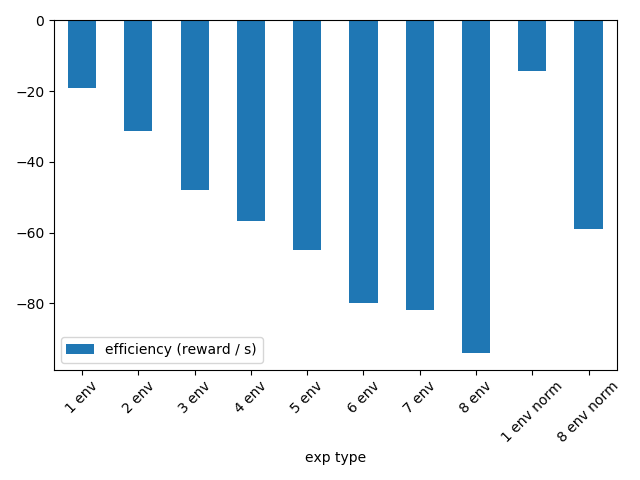
\includegraphics[width=0.7\textwidth]{../efficiency_by_exp_type.png}
\caption{Efficiency vs env type.}
\end{figure}




\section{Findings summary}

\begin{enumerate}
  \item Increasing the nb of env tend to harm the performance.
  \item Normalising helps.
  \item Normalising increases the training time.
  \item The most efficient is to use one env and to normalise
  \item I NEED TO RE RUN THIS WITH MORE TIME STEPS.
\end{enumerate}
 


\end{document}